\chapter{Потоковые шифры}\label{chapter-stream-ciphers}
\selectlanguage{russian}

Потоковые шифры осуществляют посимвольное шифрование открытого текста. Под символом алфавита открытого текста могут пониматься как отдельные биты (побитовое шифрование), так и байты (побайтовое шифрование). Общий вид большинства потоковых шифров приведён на рис.~\ref{fig:stream-cipher}.

\begin{figure}[hb]
	\centering
	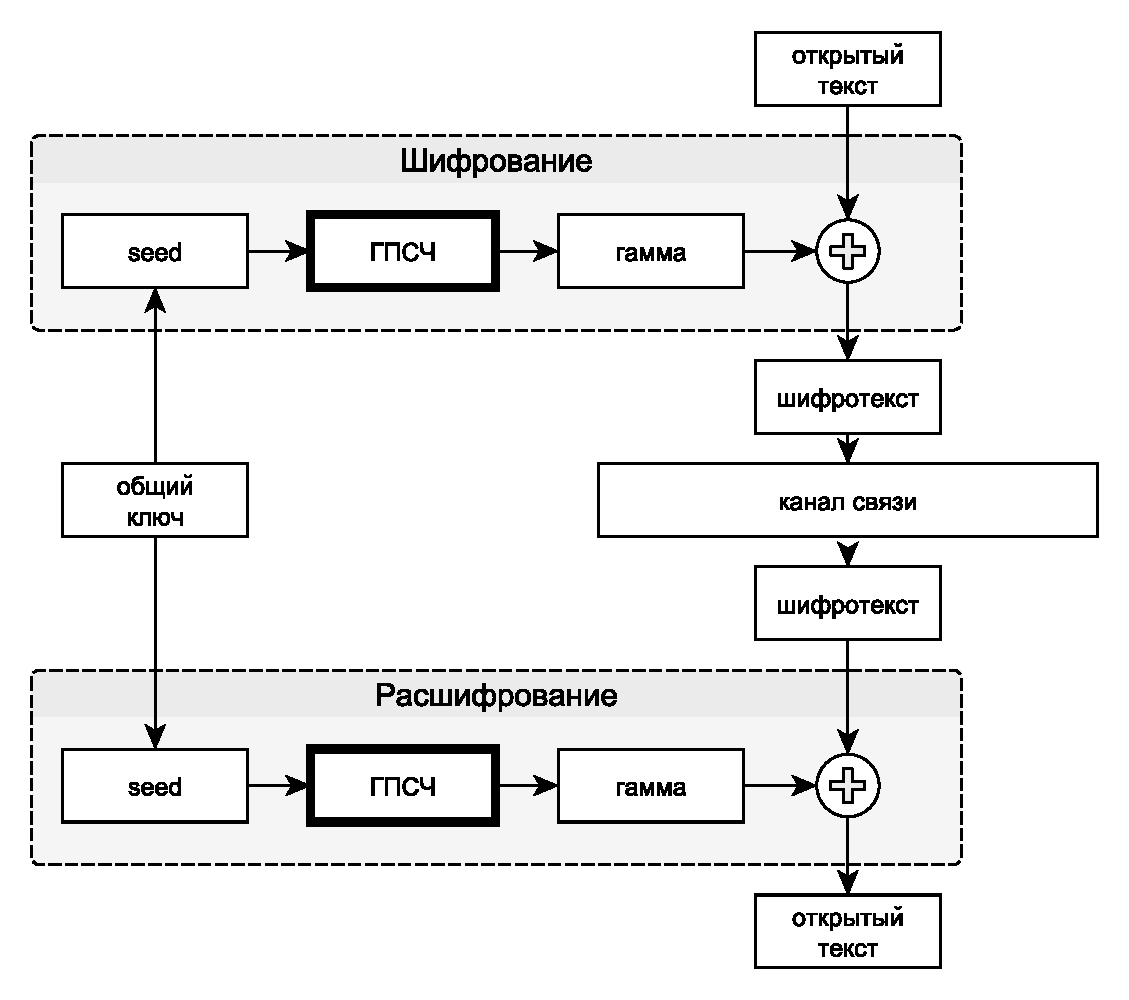
\includegraphics[width=0.66\textwidth]{pic/stream-cipher}
  \caption{Общая структура шифрования с использованием потоковых шифров}
  \label{fig:stream-cipher}
\end{figure}

\begin{itemize}
	\item Перед началом процедуры шифрования отправитель и получатель должны обладать общим секретным ключом.
	\item Секретный ключ используется для генерации инициализирующей последовательности (\langen{seed}) генератора псевдослучайной последовательности.
	\item Генераторы отправителя и получателя используются для получения одинаковой псевдослучайной последовательности символов, называемой \emph{гаммой}\index{гамма}. Последовательности одинаковые, если для их получения использовались одинаковые ГПСЧ, инициализированные одной и той же инициализирующей последовательностью, при условии, что генераторы детерминированные.
	\item Символы открытого текста на стороне отправителя складываются с символами гаммы, используя простейшие обратимые преобразования. Например, побитовое сложение по модулю 2 (операция <<исключающее или>>, \langen{XOR}). Полученный шифротекст передаётся по каналу связи.
	\item На стороне легального получателя с символами шифротекста и гаммы выполняется обратная операция (для XOR это будет просто повторный XOR) для получения открытого текста.
\end{itemize}

Очевидно, что криптостойкость потоковых шифров непосредственно основана на стойкости используемых ГПСЧ. Большой размер инициализирующей последовательности, длинный период, большая линейная сложность -- необходимые атрибуты используемых генераторов.

Одним из примеров ненадёжных потоковых шифров является семейство A5\index{шифр!A5} (A5/1, A5/2), кратко рассмотренные в разделе~\ref{section:majority_generators}. Мы также рассмотрим вариант простого в понимании шифра RC4, не основанного на РСЛОС.

\section{Шифр RC4}\label{rc4}\index{шифр!RC4|(}
\selectlanguage{russian}

Шифр RC4 был разработан Роном Ривестом (\langen{Ronald Linn Rivest}) в 1987 году для компании RSA Data Security. Описание алгоритма было впервые анонимно опубликовано в телеконференции Usenet sci.crypt в 1994 году\footnote{См. раздел 17.1. <<Алгоритм RC4>> в~\cite{Schneier:2002}}.

Генератор, используемый в шифре, хранит своё состояние в массиве из 256-ти ячеек $S_0, S_1, \dots, S_{255}$, заполненных значениями от 0 до 255 (каждое значение встречается только один раз), а также двух других переменных размером в 1 байт $i$ и $j$. Таким образом, количество различных внутренних состояний генератора равно $255! \times 255 \times 255 \approx 2.17 \times 10^{509} \approx 2^{1962}$.

Процедура инициализации генератора.
\begin{itemize}
	\item Для заполнения байтового массива из 256-ти ячеек $K_0, K_1, \dots, K_{255}$ используется предоставленный ключ. При необходимости (если размер ключа менее 256 байтов) ключ используется несколько раз, пока массив $K$ не будет заполнен целиком.
	\item Начальное значение $j$ равно $0$.
	\item Далее для значений $i$ от $0$ до $255$ выполняется:
	\begin{enumerate}
		\item $j:= (j + S_i + K_i) \mod 256$,
		\item поменять местами $S_i$ и $S_j$.
	\end{enumerate}
\end{itemize}

Процедура получения следующего псевдослучайного байта $result$ (следующего байта гаммы):
\begin{enumerate}
	\item $ i := (i + 1) \mod 256$,
	\item $ j := (j + S_i) \mod 256$,
	\item поменять местами $S_i$ и $S_j$,
	\item $ t := ( S_i + S_j ) \mod 256$,
	\item $ result := S_t$.
\end{enumerate}

По утверждению Брюса Шнайера, алгоритм настолько прост, что большинство программистов могут закодировать его по памяти. Шифр RC4 использовался во многих программных продуктах, в том числе в IBM Lotus Notes, Apple AOCE, Oracle Secure SQL и Microsoft Office, а также в стандарте сотовой передачи цифровых данных CDPD. В настоящий момент шифр не рекомендуется к использованию~\cite{rfc7465}, в нём были найдены многочисленные, хотя и некритичные уязвимости~\cite{Fluhrer:Mantin:Shamir:2001,Mantin:Shamir:2002,Paul:Maitra:2007,Sepehrdad:Vaudenay:Vuagnoux:2011}.

\index{шифр!RC4|)}

